\documentclass{article}
\usepackage[left=0.85in, right=0.85in, top=0.5in, bottom=0.95in]{geometry}
\usepackage[T1]{fontenc}
\usepackage[utf8]{inputenc}
\usepackage[italian]{babel}
\usepackage{graphicx}
\usepackage{wrapfig2}
\usepackage{amsmath}
\usepackage{amssymb}
\usepackage{cases, cancel}
\usepackage{gensymb} %simboli come ° = \degree  etc etc
\usepackage{subcaption}
\usepackage{hyperref}
\hypersetup{
	colorlinks=true,
	linkcolor=blue,    
	urlcolor=blue,
	%pdfpagemode=FullScreen,
}
\urlstyle{same}
\usepackage{changepage}
\usepackage{lastpage, epstopdf}
\usepackage{fancyhdr}
\usepackage{tcolorbox}
%\usepackage{background}
\usepackage{tikz}
\usetikzlibrary{patterns}


%=======HEADER & FOOTER=======%
\def\lesson{Lezione N. 11}
\def\outcome{\textbf{Learning Outcomes:} Outcomes go here. }

\pagestyle{fancy}
\fancyhf{}
\renewcommand{\headrulewidth}{0pt}
\renewcommand{\footrulewidth}{1.4pt}
\lfoot{A.M. $\diamond$ \the\year}
\cfoot{Page \thepage}
\rfoot{\lesson}

%=======CORNELL STYLE FORMAT=======%
%\SetBgScale{1}
%\SetBgAngle{0}
%\SetBgColor{black}
%\SetBgContents{\rule{1pt}{0.85\paperheight}}
%\SetBgHshift{-1.6in}
%\SetBgVshift{-0.1in}

%=======CUSTOM BOXES=======%

\parindent 0ex

%=======BODY=======%
\begin{document}
	\setcounterpageref{secnumdepth}{0}
	\section*{Parte 7} %Date: \hrulefill}
%	\begin{tcolorbox}{\outcome}\end{tcolorbox}

\begin{adjustwidth}{2in}{}  
	
\textbf{{\Large Criteri di resistenza per carichi statici}} \mbox{} \newline
		Il fine della progettazione sarà anche quello di prevedere ed evitare il guasto del componente, questo può essere dato da fratture, rotture e snervamento, ovvero tutte quelle condizioni per le quali non si avrà un corretto funzionamento. \newline 
		
		Ci si occupa ora della sola resistenza ai carichi statini, ovvero quelle sollecitazioni associabili ad $\vec{F}, \vec{M}$ i cui descrittori statici saranno costanti e non variabili nel tempo in modulo, direzione, verso e punti di applicazione. \newline 
		
		A seguito dell'applicazione di un carico statico va verificata la resistenza del componente meccanico, ma da cosa dipende la resistenza ai carichi statici? Dal materiale stesso, dall'ambiente di esercizio, dai trattamenti termici, dalle lavorazioni tecnologiche, dalla presenza di zone critiche associabili a brusche variazioni di forma sede di concentrazioni di tensione e dalla tipologia di carico: differenti tipologie di carico porteranno a diverse risposte del componente. \newline 
		
		Le verifiche si esporranno dunque in termini di disuguaglianze tra scalari, di confronto tra due entità: tra il carico che si applica alla struttura e la resistenza del componente. 
		
		Carichi applicati generano distribuzioni di tensioni ottenibili dal tensore delle tensioni, ma per geometrie reali come si può scrivere tale tensore? Tanto più è complessa la geometria tanto più è complicato tradurre i carichi applicati in tensori: bisogna ricondursi a modelli semplificativi. 
		
		Per quanto riguarda la resistenza del materiale risulta invece complesso ottenere un valore realistico perfettamente determinato, l'approccio deterministico è infatti associato un elevato grado di incertezza a cui è necessario associare un coefficiente di sicurezza. Più efficace sarebbe verificare il componente nelle condizioni reali, ben differenti da quelle laboratoriali o simulative, ma sarebbe possibile per piccoli lotti e in ogni caso non ci si libererebbe da una distribuzione di probabilità data da un approccio statistico. \newline 
		
		Il problema dell'affidabilità meccanica è affrontato in maniera affidabilistica secondo leggi statistiche stocastiche. 
		
		In prima approssimazione viene usato un approccio deterministico con un confronto netto tra le grandezze di esercizio e quelle di verifica attraverso opportuni coefficienti di sicurezza che restituiranno i margini di esercizio. 
		
		La sperimentazione sul componente è un approccio che risulta sempre più pratico e sicuro, definirà se la progettazione è corretta o meno, ma di contro è estremamente costoso perciò verrà utilizzato per componenti a basse produzioni, in piccole serie, la cui importanza è elevata per motivi economici, prestazionali o di sicurezza e quindi si procederà realizzando il prototipo che poi verrà testato e verificato. 
		
		Per le normali produzioni meccaniche non si è raramente in tali condizioni economiche di vantaggio per cui l'approccio che andrà per la maggiore sarà quello analitico, deterministico, in prima approssimazione sempre corretto. \newpage 
		
		\textbf{{\Large Verifiche di funzionamento}}\newline 
		Primo step che un progettista meccanico deve sempre precorrere nella realizzazione di un progetto meccanico è la \textbf{Verifica Statica}. Nel momento in cui invece si lavorerà al di fuori delle normali condizioni di design interesserà più non tanto che il componente continui a lavorare ma che non ceda pericolosamente e la verifica che si andrà ad effettuare sarà a cedimento. \newline 
		
		\begin{center}
		\textit{	L'azione di un carico statico non deve portare il materiale al raggiungimento della tensione ultima.} \newline
		\end{center}
	
		Cosa differenzia un materiale duttile da un materiale fragile? Un AISI306, un FE340 presentano un comportamento chiaramente ed evidentemente duttile, mentre materiali come leghe e ghise sono più di difficile interpretazione a causa della composizione chimica, della quantità di precipitati e della temperatura di esercizio.
		
		 Si definisce quindi il comportamento del materiale in termini di allungamento ultimo a rottura ad una determinata temperatura ambientale: 
		 
		 Un materiale per essere duttile deve presentare un allungamento ultimo a rottura superiore al 5\%, altrimenti è fragile. \newline 
		 
		 Attenzione a non "etichettare" i materiali, il comportamento sinora analizzato si evidenza a temperatura ambiente in condizioni di esercizio standard, lo stesso duttile acciaio a temperature criogeniche ha comportamento fragile, così come nelle applicazioni nucleari a seguito di bombardamento neutronico.  
		 
		 La resistenza di un materiale dipende dalle condizioni ambientali a cui esso è sottoposto. \newline
		 
		 Attraverso le verifiche a rottura e snervamento il componente ha passato il suo test d'ingresso, ora in dipendenza delle applicazioni di dovranno magari verificare gli spostamenti: un albero che si piega così tanto da non poter più riuscire a far toccare due ruote dentate non è rotto, ma certamente non funziona più e così oltre alle verifiche statiche e di resistenza si dovranno prevedere verifiche funzionali. \newline 
		 
		 Sugli stessi alberi di trasmissione si verifica sia la freccia massima per garantire che i componenti rimangano calettati, sia le rotazioni sui cuscinetti, che lavorano solamente all'interno di uno specifico range di funzionamento. 
		 
		 Si effettueranno verifiche sulle condizioni, ad esempio se il carico è di compressione il componente può cedere per instabilità flessionale ancor prima che avvenga la criticità con carico statico, a causa di imperfezioni di forma o a causa di un carico non perfettamente centrato. 
		 
		 Si verificherà poi la fatica, ovvero i carichi ciclici nel tempo; la concentrazione delle tensioni; i difetti, sedi questi di innesco del danneggiamento che porta a fratture fragili anche materiali duttili; il creep viscoelastico, che sotto determinate caratteristiche di carico e temperatura porta ad una deformazione variabile nel tempo; si prevederanno verifiche a urti magari per serbatoi e si potrà addirittura considerare il suono emessi dal componente sotto determinate condizioni. \newline 
		 
		 Tutte queste verifiche si trasformano in una disuguaglianza tra scalari:
		 \[\sigma_{\text{applicata}}\leq \sigma_{\text{ammissibile}}\]
		 Dove la tensione ammissibile non sarà altro che la tensione di snervamento o di rottura, ottenute magari da prove di trazione, divisa per un opportuno coefficiente di sicurezza.\newline 
		 
		 Finché le condizioni di carico sono monodimensionali e il tensore delle tensioni si trasforma in uno scalare, non ci si pone problemi a far rispettare la disuguaglianza, ma quando le condizioni di carico diventano reali, allora il tensore di De Saint Venant si riempie di altri termini, per cui risulta più complicato trasformarlo in scalare. 
		 
		 Ad esempio, un albero di trasmissione è sempre sottoposto a flessione e momento torcente, per cui, valendo la sovrapposizione degli effetti, come faccio a tradurre questo tensore
		 \[\left[\begin{array}{ccc}
		 	0 & 0 & \tau_{xz} \\
		 	0 & 0 & \tau_{yz} \\
		 	\tau_{xz} & \tau_{zy} & \sigma_z
		 \end{array}\right]\]
	 	In uno scalare? In caso di sollecitazioni pluridimensionali è necessario ricavare una
	 	tensione monodimensionale equivalente o
	 	ideale 
	 	\[\sigma_i = (\sigma_1, \sigma_2, \sigma_3)\]
	 	
	 	\textbf{{\Large Criteri di resistenza}}\newline 
	 	 I criteri di resistenza in base al materiale e alla sollecitazione vanno ad osservare quale sia il meccanismo, all'interno del materiale, che porta a rottura o a snervamento. 
	 	
	 	Esistono numerose teorie sui meccanismi che portano al guasto o al cedimento del componente, i
	 	diversi modelli di guasto proposti sono stati confrontati con le evidenze sperimentali definendo un criterio
	 	di scelta dettato da vari fattori tra cui il più determinante è sicuramente il comportamento del materiale, se duttile o fragile. 
	 	
	 	Perché si usano criteri diversi per comportamenti diversi? Perché semplicemente il meccanismo che porta a rottura il materiale è dipendente dal materiale stesso. 
	 	
	 	Si useranno allora i criteri di Tresca, Von Mises e Mohr-Coulomb per materiali duttili (l'ultimo se il materiale identificherà comportamenti diversi a trazione e compressione) e per i materiali fragili si utilizzeranno i criteri di Rankine, Mohr-Coulomb fragile e Mohr-Coulomb modificato. \newline 
	 	
	 	\textbf{{\Large Criterio della Massima Tensione Tangenziale di Tresca}} \newline 
	 	Il criterio più immediato da comprendere è quello di Tresca, che deriva da una semplice osservazione: un provino duttile mentre si traziona e si striziona rende visibile ad occhio nudo delle linee di scorrimento a 45\degree: è in questa giacitura che si manifesta la massima tensione tangenziale $\tau$. \newline
	 	
	 	Si visualizzi ora il tensore delle tensione di questa sollecitazione sui cerchi di Mohr, cos'era la rappresentazione di Mohr? Una rappresentazione grafica delle forme che può assumere il tensore delle tensioni in un punto al variare delle direzioni di rappresentazione del tensore. 
	 	
	 	Stante uno stato tensionale in un punto, se si utilizza come rappresentazione gli assi principali si individuano le tre tensioni principali $\sigma_1 ~ \text{massima}, \sigma_2 ~ \text{intermedia}, \sigma_3 ~ \text{minima}$ come intersezioni delle tre circonferenze con l'asse delle $\sigma$, nelle direzioni principali inoltre le $\tau$ sono nulle. 
	 	
	 	\begin{figure}[H]
	 		\centering
	 		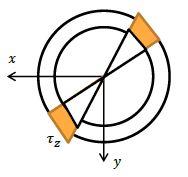
\includegraphics[width=0.5\linewidth]{immagini/screenshot001.1}
	 		\label{fig:screenshot001.1}
	 	\end{figure}
	 		 	
	 	Nel caso di tensione monoassiale di trazione $\sigma_1=N/A$ e $\sigma_2=\sigma_3=0$. In queste condizione si ha un cerchio di Mohr da $\sigma_1$ a $\sigma_3$ ed un punto che collassa in zero coincidente con le $\sigma_2$ e $\sigma_3$.
	 	
	 		 	\begin{figure}[H]
	 		\centering
	 		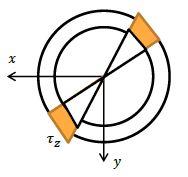
\includegraphics[width=0.5\linewidth]{immagini/screenshot001.2}
	 		\label{fig:screenshot001.2}
	 	\end{figure}
	 	
	 	C'è solo una circonferenza, ed è la massima. 
	 	
	 	Come si consulta il diagramma di Mohr? Mettendosi al centro si possono conoscere il valori che assumono $\tau$ e $\sigma$ alla rotazione intorno ad uno dei sue assi principali. 
	 	
	 	In questo caso si ruoti intorno ad $x$ gli assi $z$ ed $y$. 
	 	
	 	Una rotazione sul piano di Mohr corrisponde a metà di un angolo di rotazione vera della giacitura, per cui se si ruota di 45\degree la giacitura, si ottiene un angolo di 90\degree sul piano di Mohr, ed è proprio lì che sarà la massima tensione tangenziale $\tau$ tale per cui se si muove di un altro grado la giacitura, comincerà a decrementare. \newline
	 	
	 	Cos'è che suggerisce allora Tresca? Che sono le $\tau$ in un materiale duttile a creare criticità e quindi a portare a rottura, vuol dire che non sono le $\sigma$ da monitorare e confrontare, sono le $\tau$ che vanno confrontate con una tensione tangenziale ammissibile, sono queste ora le tensioni massime che hanno portato a snervamento il provino nella macchina di trazione. \newline 
	 	
	 	Osservando il diagramma di Mohr ci si accorge allora che la condizione di $\tau_{max}$ si ha proprio in corrispondenza del raggio della circonferenza, questo dato da $\sigma_1/2$: la $\tau_{max}$ è il massimo raggio delle tre circonferenze di Mohr. \newline 
	 	
	 	La tensione equivalente di Tresca si può scrivere come il valore massimo delle differenze tra le tensioni principali:
	 	\[\tau_{max} = \max \left\{ \left|\sigma_1-\sigma_2\over 2\right|; \left|\sigma_1-\sigma_3\over 2\right|;      \left|\sigma_2-\sigma_3\over 2\right|\right\} \leq \tau_{amm} = {\sigma_{amm}\over2}\]
	 	E dunque, in termini di tensione principale: 
	 	\[\sigma_{eq} = \max \left\{ \left|\sigma_1-\sigma_2\right|; \left|\sigma_1-\sigma_3\right|;      \left|\sigma_2-\sigma_3\right|\right\} \leq \sigma_{amm}\]
	 	Si cerca ora una rappresentazione grafica di tutto ciò che sia anche facile da leggere. 
	 	
	 	Nello spazio tridimensionale dato da $\sigma_1, \sigma_2, \sigma_3$ si può definire un volume che contenga tutti gli stati tensionali in condizioni elastiche ed un volume al di fuori che rappresenti le condizioni critiche, come rottura, snervamento o gusto. \newline 
	 	
	 	Mettere un criterio di resistenza significa imporre una frontiera elastica all'interno della quale il componente è in condizioni di sicurezza: se uno stato tensionale appartiene all'interno della frontiera allora gli si associano condizioni elastiche e la verifica è superate, se tale stato appartiene alla frontiera cominciano ad insorgere criticità, se invece lo stato tensionale è al di fuori di tale frontiera la verifica non è superata. 
	 	
	 	Che forma ha questa frontiera? Si sezioni il volume con un piano rappresentato da $\sigma_3=0$ e ci si chieda come si comporta il limite elastico di Tresca in caso di tensione piana:
	 	\[\sigma_{eq} = \max \left\{ \left|\sigma_1-\sigma_2\right|; \left|\sigma_1\right|;      \left|\sigma_2\right|\right\} \leq \sigma_{amm}\]
	 	Limitato superiormente e inferiormente da $\pm\sigma_1$ e $\pm\sigma_2$ e lateralmente da $\pm(\sigma_1-\sigma_2)$ la frontiera elastica di Tresca è un esagono.
	 	
	 	\begin{figure}[H]
	 		\centering
	 		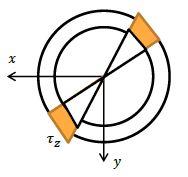
\includegraphics[width=0.4\linewidth]{immagini/screenshot001}
	 		\label{fig:screenshot001}
	 	\end{figure}
	 	 	
	 	Tale criterio si applica per materiali duttili a comportamento identico a trazione e compressione. \newline 
	 	
	 	Nel caso di sole tensioni tangenziali il criterio può essere riscritto come:
	 	\[\tau_{max}\leq\tau_{amm} = 0.5\sigma_{amm}\]
	 	Questo criterio, mentre da una parte offre un'elevata conservatività, dall'altra diviene utilizzabile solo se il tensore delle tensioni è ricondotto alle tensioni principali.  
	 	
	 	C'è un altro criterio che magari può evitare la trasformazione del tensore in principale? \newline 
	 	
	 	\textbf{{\Large Criterio dell'Energia di Distorsione di Von Mises}} \newline 
	 	Questo criterio sancisce che lo snervamento del materiale avviene quando si introduce nello stesso una quantità di energia di distorsione specifica (per unità di volume), pari a quella che si manifesta nel provino posto a trazione o compressione semplice. \newline 
	 	
	 	Cos'è questa energia di distorsione? Si definisca prima di tutta la tensione idrostatica. 
	 	
	 	Questo criterio deriva dall'osservazione di materiali duttili in condizione di sollecitazione idrostatica, condizione questa per la quale la tensione applicata è uniforme in tutte le direzioni: $\sigma_1=\sigma_2=\sigma_3$. 
	 	
	 	I materiali duttili soggetti a questo tipo di sollecitazione presentano una deformazione di sola dilatazione volumica senza variazione di forma, si evidenzia inoltre come lo stesso materiale risulti più resistente a questo tipo di sollecitazione piuttosto che a quella di trazione semplice. \newline 
	 	
	 	Se Tresca diceva che il materiale duttile scorre a 45\degree e quindi la $\tau$ è lì che è massima, con Von Mises dipenderà anche da com'è che si deforma il materiale, non è più solo un concetto di direzione di scorrimento. \newline 
	 	
	 	Se la sollecitazione porta a sola dilatazione, quindi ad una variazione di volume, allora il materiale sarà più resistente di quando lo si andrà a distorcere. 
	 	
	 	L'energia di deformazione idrostatica più l'energia di deformazione distorsiva daranno insieme l'ammontare di energia di deformazione, del lavoro di deformazione necessario, questo esprimibile come, sotto l'ipotesi di tensioni scritte in forma principale: 
	 	\[U = \int\sigma d\varepsilon = {1\over2}\sigma\varepsilon = {1\over2E}[\sigma_1^2 + \sigma_2^2 + \sigma_3^2 + 2\nu(\sigma_1\sigma_2 + \sigma_1\sigma_3 + \sigma_2\sigma_3) ]\]
	 	L'infinitesimo cubo materiale è soggetto a $\sigma_1, \sigma_2, \sigma_3$ questi scomponibili come una sovrapposizione di una tensione media $\sigma_m$ idrostatica più una composizione di tensioni atte a restituire la condizioni di partenza.
	 	
	 	\begin{figure}[H]
	 		\centering
	 		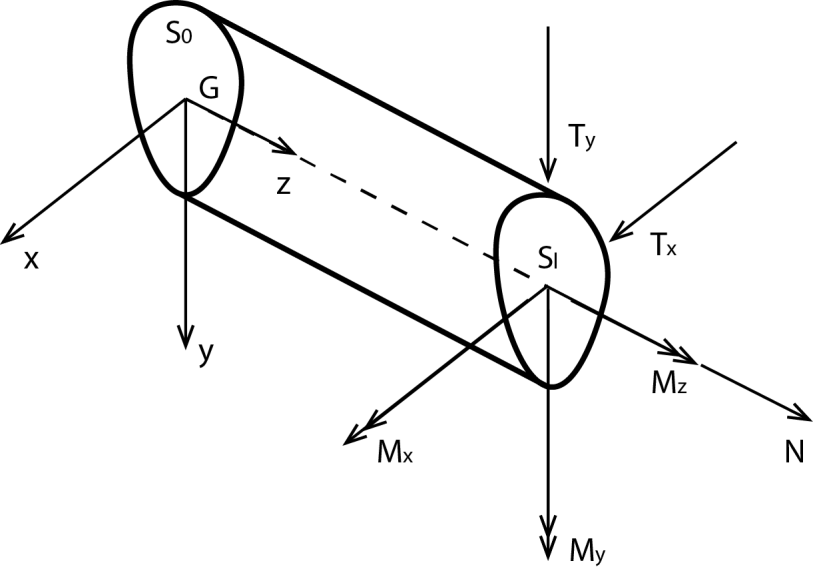
\includegraphics[width=0.5\linewidth]{immagini/screenshot002}
	 		\label{fig:screenshot002}
	 	\end{figure}	 	
	 	
	 	Ora, se il primo ed il secondo sono generici stati tensionali, sarà il terzo ad essere quello distorsivo, associato alla distorsione, la cui energia $U_D$ potrà essere ricavata attraverso una differenza tra quella totale $U$ e quella idrostatica $U_I$:
	 	\begin{eqnarray*}
	 		\sigma_m = {\sigma_1+\sigma_2+\sigma_3\over3} \hspace{1cm} U_I = {3\sigma_m^2\over2E}(1-2\nu) \\	 		
	 		U_I = {1-2\nu\over6E}[\sigma_1^2 + \sigma_2^2 + \sigma_3^2 + 2(\sigma_1\sigma_2 + \sigma_1\sigma_3 + \sigma_2\sigma_3)] 	 		
	 	\end{eqnarray*}
 		\[U_D = U-U_I = {1-\nu\over3E}[\sigma_1^2 + \sigma_2^2 + \sigma_3^2 + (\sigma_1\sigma_2 + \sigma_1\sigma_3 + \sigma_2\sigma_3)] \]
	 	Cosa afferma Von Mises? Che quando questa energia è pari all'energia di distorsione necessaria a portare allo snervamento il materiale, avviene lo snervamento. \newline 
	 	
	 	Particolarizzo quindi tale equazione nel caso di trazione, con $\sigma_2=\sigma_3 = 0$:
	 	\[U_D^{snerv} = {1-\nu\over3E}\sigma_1^2 = {1-\nu\over3E}\sigma_{amm}^2 \]
	 	Ecco l'energia di distorsione associata all'incipiente snervamento per prove di trazione, quando le due energie saranno uguali anche nel caso reale si avrà snervamento, si giunge in questo modo alla tensione equivalente di Von Mises: 	 	
	 	\begin{eqnarray*}
	 	U_D^{snerv} = U_D \Rightarrow \cancel{{1-\nu\over3E}}\sigma_{amm}^2 = \cancel{{1-\nu\over3E}}[\sigma_1^2 + \sigma_2^2 + \sigma_3^2 + 2(\sigma_1\sigma_2 + \sigma_1\sigma_3 + \sigma_2\sigma_3)] \\
	 	\sigma_{eq} = \sqrt{\sigma_1^2 + \sigma_2^2 + \sigma_3^2 + (\sigma_1\sigma_2 + \sigma_1\sigma_3 + \sigma_2\sigma_3)} \leq \sigma_{amm}
	 	\end{eqnarray*}	
 		È un approccio molto più accurato rispetto a quello di Tresca, ma più complesso da ricavare. 
 		
 		Un conto sarà dunque usare una sottrazione di tensioni principali come in Tresca, un altro sarà utilizzare Von Mises, questo si configura perciò come un criterio adatto alla singola verifica, se si deve invece introdurre un criterio all'interno di un nuovo modello si preferirà Tresca, che dal canto suo possiede una buona semplicità di calcolo e ha un'elevata conservatività (sicurezza). 
 		
 		Tresca esclude molti più stati tensionali. Rappresentando l'insieme di Von Mises per una sollecitazione piana si ottiene un'ellisse nella quale l'esagono di Tresca è inscritto: Tresca definisce un insieme di soluzioni valide più piccolo. Se per Von Mises alcune condizioni di carico possono sussistere, per Tresca no, sarà necessario allora ridimensionare il componente (più costoso ma necessario?) sapendo che ci si metterà ancor più in sicurezza.
 		\[\sigma_{eq} = \sqrt{\sigma_1^2 + \sigma_2^2 + \sigma_1\sigma_2 } \leq \sigma_{amm}\]
 		
 		\begin{figure}[H]
 			\centering
 			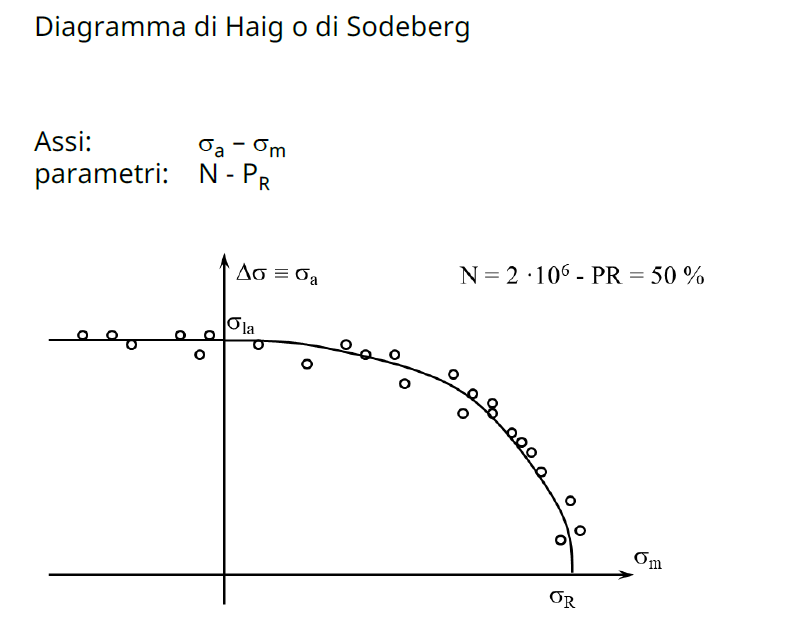
\includegraphics[width=0.5\linewidth]{immagini/screenshot003}
 			\label{fig:screenshot003}
 		\end{figure}
 				 
 		\begin{itemize}
 			\item Criterio accurato $\rightarrow$ Von Mises
 			\item Criterio conservativo + calcoli semplici $\rightarrow$ Tresca
 		\end{itemize}
 		Von Mises dal canto suo permette però di poter utilizzare un tensore espresso come non principale.
 		
 		Se a ritroso si mettono le formulazioni di Mohr nella tensione equivalente appena trovata, si ottiene:
 		\[\sigma_{eq} = \sqrt{\sigma_x^2 + \sigma_y^2 + \sigma_x\sigma_y +3\tau_{xy}^2} \leq \sigma_{amm}\]
 		Dove nel caso tridimensionale si aggiungerà un $\sigma_z^2$ i termini mutui in $\sigma$ e le altre due $\tau$ mancanti. \newline 
 		
 		Per sollecitazioni piane di puro taglio in cui $\sigma_x = \sigma_y = 0$ resisteranno solo le $\tau$:
 		\[\sigma_{eq} = \sqrt{3\tau_{xy}^2} \l= \sigma_{amm} \Rightarrow \tau_{xy} = {\sigma_{amm}\over\sqrt{3}} = 0.577\sigma_{amm} \]
 		Von Mises è più tollerante di un 15\% rispetto a Tresca. 
 		
 		Infatti la presenta di una $\tau_{max}$ in questo caso corrisponderà ad un tensore del genere:
 		\[\left[\begin{array}{ccc}
 			0 & \tau_{xy} & 0 \\
 			\tau_{yx} & 0 & 0 \\
 			0 & 0 & 0
 		\end{array}\right]\] 
 		Che corrisponderà a:
 		\[\left[\begin{array}{ccc}
 			\sigma_1 & 0 & 0 \\
 			0 & -\sigma_1 & 0 \\
 			0 & 0 & 0
 		\end{array}\right]\] 
 		Sull'ellisse di Von Mises altro non è che la bisettrice (a 45\degree) del secondo e quarto quadrante, l'intersezione di questa con l'esagono darà la tensione massima di Tresca $0.5\sigma$ mentre l'intersezione con l'ellisse darà la tensione massima di Von Mises $0.577\sigma$, la differenza tra i due è esattamente il 15\% di tolleranza in più che ha Von Mises. \newline 
 		
 		\textbf{{\Large Criterio di Mohr-Coulomb }} \newline 
 		Per materiali caratterizzati da un limite a trazione e compressioni diversi, Mohr-Coulomb è la scelta migliore.
 		
 		Per questo criterio si procede caratterizzando il materiale sono a trazione, solo a compressione e solo a taglio, si rappresenteranno poi sul piano di Mohr le caratteristiche così rilevate. 
 		
 		La curva di inviluppo che contiene le tre circonferenze così ottenute è dalla definizione la curva limite del materiale non sul piano $\sigma_1\sigma_2\sigma_3$ ma sul piano di Mohr. 
 		
 		Per una qualunque condizione di carico se le tre circonferenze stanno tutte all'interno della curva di Mohr la condizione è non critica e sarà di sola sollecitazione elastica, se iniziano ad essere tangenti (come rappresentato) la situazione inizia a divenire critica, e se infine la superano, si sta oltre lo snervamento. 
 		
 		\begin{figure}[H]
 			\centering
 			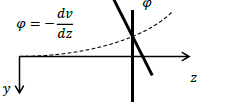
\includegraphics[width=0.3\linewidth]{immagini/screenshot004}
 			\label{fig:screenshot004}
 		\end{figure}
 		
 		
 		Per ottenere tale inviluppo, come detto, è necessario caratterizzare il materiale a trazione, a compressione e a taglio, ed è complesso. \newline 
 		
 		L'evoluzione di questo criterio è data da Coulomb che a differenza di Mohr, prevede la curva di inviluppo come rette. 
 		
\begin{figure}[H]
	\centering
	\label{fig:screenshot005}
	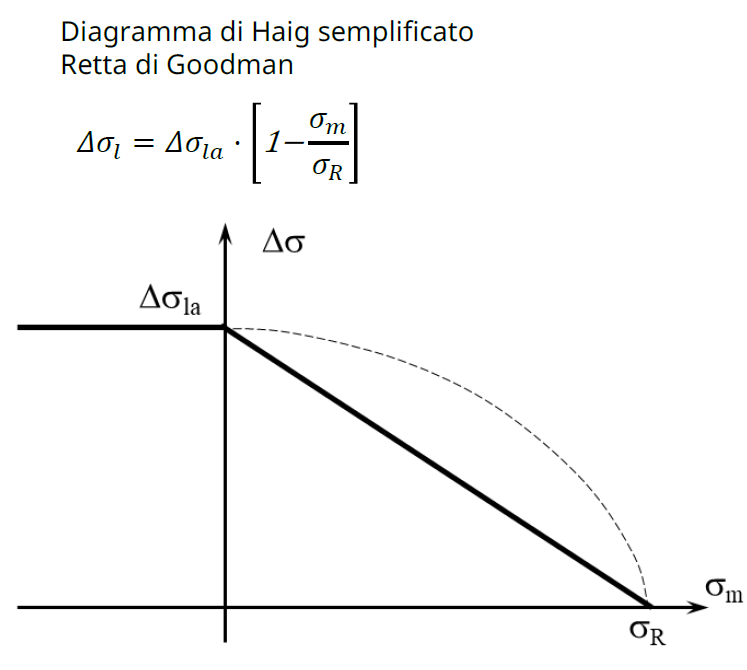
\includegraphics[width=0.3\linewidth]{immagini/screenshot005}
\end{figure}
 				
 		Come si ricavano? Attraverso una prova di sola trazione (circonferenza a destra) si porta il materiale allo snervamento a trazione $\sigma_t$, con una prova a compressione (circonferenza a sinistra) si porta il materiale allo snervamento a compressione $\sigma_c$, notare come in queste sollecitazioni, essendo monoassiali, si avrà una sola tensione principale, rispettivamente o $\sigma_t$ 0 $\sigma_c$, mentre le altre due saranno nulle. \newline 
 		
 		Le rette tangenti le circonferenze tratteggiate rappresentano così la curva di inviluppo di Mohr-Coulomb. 
 		
 		Si ha criticità quando la circonferenza massima dello stato tensionale è tangente a queste linee di inviluppo. 
 		
 		Nella figura è stata quindi a ragione rappresentata solo la circonferenza che va da $\sigma_1$ a $\sigma_3$, la presenza di una $\sigma_2$ intermedia non poterà contributo non avendo questa tangenza con le linee di inviluppo. 
 		
 		L'attenzione perciò è sempre focalizzata sulla circonferenza più grande. \newline 
 		
 		Matematicamente questa condizione si traduce nella relazione: 
 		
 		$\sigma_1$ normalizzato rispetto alla sua tensione ammissibile a trazione MENO $\sigma_3$ normalizzato rispetto alla sua tensione ammissibile a compressione maggiore o uguale ad uno.
 		\[{\sigma_1\over\sigma_{amm,t}} - {\sigma_3\over\sigma_{amm,c}}\geq 1\]
 		
 		\textbf{{\Large Sperimentazione}} \newline 
 		\begin{figure}[H]
 			\centering
 			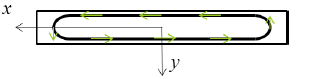
\includegraphics[width=0.65\linewidth]{immagini/screenshot006}
 			\label{fig:screenshot006}
 		\end{figure}
 		
 		
 		I punti su questo grafico identificano lo snervamento, e quindi la condizione di criticità del materiale. 
 		
 	 	Sperimentalmente per materiali duttili tali punti si attestano con buona approssimazione all'interno dell'ellisse di Von Mises e al di fuori dell'esagono di Tresca, sono i punti dove si è snervato il materiale duttile. \newline 
 		
 		Per ghise grigie si vede bene come il comportamento risulti a cavallo tra il duttile ed il fragile: i criteri fin'ora analizzati non funzionano correttamente.
 		
 		Tresca darebbe per sicuro delle condizioni che in realtà sono critiche e delle condizioni addirittura molto al di fuori delle condizioni critiche di Von Mises e Tresca, ottenendo un'estrema conservatività del materiale. 
 		
 		Potrebbe in questo caso andar meglio un approccio con Mohr-Coulomb in un grafico che terrà conto del diverso comportamento a trazione e compressione: si immagini ad esempio un materiale che abbia pari resistenza a trazione ricalcando Tresca ed una maggiore resistenza a compressione, il grafico manterrebbe certo una forma esagonale ma sarebbe decentrato e deformato rispetto a quello di Tresca.
 		
\begin{figure}[H]
	\centering
	 		\begin{tikzpicture}[>=latex]
 			%%%	Help Lines
% 			\draw [thin, help lines] (0,0) grid (10,10);
% 			\foreach \x in {0,...,10}
% 			\draw (\x cm,1pt) -- (\x cm,-1pt) node[anchor=north] {$\x$};
% 			\foreach \y in {0,...,10}
% 			\draw (1pt,\y cm) -- (-1pt,\y cm) node[anchor=east] {$\y$};
 			%%%	Disegno	
 			\draw[thick, ->] (0,5) -- (11,5) node [pos = 1, right] {$\sigma_1$};
 			\draw[thick, ->] (5,0) -- (5,11) node [pos = 1, above] {$\sigma_2$};
 			\draw[thick, dashed](5,8) -- (8,8) -- (8,5) -- (5,2) -- (2,2) -- (2,5) -- (5,8);
 			\draw[thick, red](5,8) -- (8,8) -- (8,5) -- (0,1) -- (-3,1) -- (-3,4)  -- (5,8);			
 		\end{tikzpicture}
\end{figure}
 		
 		Nasce così la necessità di studiare nuovi criteri per materiali fragili. \newpage
 		
 		\textbf{{\Large Criterio della Tensione Principale di Rankine}} \newline 
 		Tale criterio sancisce che la rottura avviane quando nel componente la più grande delle tensioni principali raggiunge il suo valore limite.
 		\begin{eqnarray*} 
 			\sigma_{max} = \max\left\{\sigma_1; \sigma_2; \sigma_3\right\} \leq \sigma_{amm,t}\\
 			 \sigma_{min} = \min\left\{\sigma_1; \sigma_2; \sigma_3\right\}\geq \sigma_{amm,c} 			
 		\end{eqnarray*}
 		Nello spazio tridimensionale delle tensioni principali, la superficie limite di rottura corrisponde ad un cubo
 		orientato secondo gli assi.
 		
 		La rappresentazione di tale volume nel piano $ \sigma_3 = 0 $ descrive un quadrato decentrato rispetto all'origine,
 		essendo tipicamente la tensione di rottura a compressione superiore alla tensione di rottura a trazione.
 		
 		\begin{figure}[H]
 			\centering
 			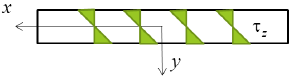
\includegraphics[width=0.3\linewidth]{immagini/screenshot007}
 			\label{fig:screenshot007}
 		\end{figure}
 		
 		
 		Riguardando il grafico sperimentale poco sopra, si intuisce subito come questo criterio non funzioni assolutamente per materiali duttili, osservando il quadrato tratteggiato, questo non dà alcuna indicazione per i materiali per cui lo snervamento cade all'interno del quarto quadrante, li darebbe tutti per assurdo in sicurezza. 
 		
 		Fornisce tuttavia un ottimo criterio per materiali fragili. \newline 
 		
 		Nel caso di taglio puro:
 		\[\tau_{max}=\sigma_1=\sigma_{amm}\]
 		
 		\textbf{{\Large Criterio di Mohr-Coulomb modificato}} \newline 
 		Valido per materiali fragili. La modifica consiste nel considerare anche un prolungamento del diagramma sperimentale. 
 		
 		Vengono a crearsi così nuove relazioni per meglio cogliere evidenze sperimentali, atte queste a compensare le porzioni di grafico nel secondo e nel quarto quadrante, estendendo la zona di sicurezza. 
 		
 		\begin{figure}[H]
 			\centering
 			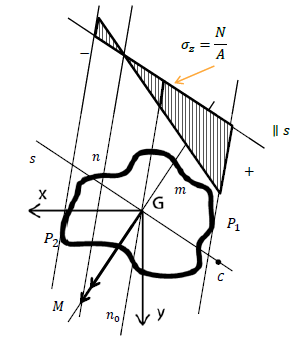
\includegraphics[width=0.95\linewidth]{immagini/screenshot008}
 			\label{fig:screenshot008}
 		\end{figure}
 		
 		In principio fu il criterio di Tresca, questo nasceva esclusivamente da un'evidenza sperimentale a cui si dava un significato teorico: negli scorrimenti a 45\degree ci sono le tensioni tangenziali massime e sono queste allora a ad essere la causa della rottura; fino ad arrivare a quest'ultimo criterio che insegue empiricamente l'evidenza sperimentale definendo una legge metrica. \newline 
 		
 		\textbf{{\Large Scelta del criterio}} \newline 
 		Qual è il processo logico che ci spinge a seguire un determinato criterio di resistenza? 
 		
 		In questo diagramma si considera MCF come Mohr-Coulomb con tensione ammissibile a rottura e MCD come Mohr-Coulomb con tensione ammissibile a snervamento, invece per Mohr modificato si intende la curva allargata atta a prendere i dati sperimentali. Le $S$ sono i carichi di snervamento per i quali ci si chiederà, per un comportamento duttile, se sono uguali a trazione e compressione. 
 		
 	\end{adjustwidth}
 	\begin{figure}[H]
 	\includegraphics[scale=0.75,page=14]{07_fcm_2022}
 	\end{figure}
 	\begin{adjustwidth}{2in}{}
 		
 		
 		
 		
 		
 		
 		
 		
	 	
	 	
	 	
	 	
	 	
	 	
	 	
		 
		 
		 
	\newpage
	{\Large \textbf{NOTE}}
%	\vfill
%\begin{tcolorbox}[height=4.5cm]
%	This box has a height of 4.5cm.
%\end{tcolorbox}

%DA DECOMMENTARE PER AVERE LA VERSIONE STAMPABILE A DUE PAGINE 	
%	\newpage
%		\null
%		\vfill
%\begin{tcolorbox}[height=4.5cm]
%	This box has a height of 4.5cm.
%\end{tcolorbox}
		\end{adjustwidth}

\end{document}